\chapter{Architecture and Design}
\label{ch:architecture}

This chapter presents the architectural design of the Linux Process Manager, including high-level system architecture, module organization, data structures, concurrency model, and design patterns employed.

\section{System Architecture Overview}

The Linux Process Manager follows a modular, layered architecture that separates concerns and enables independent development and testing of components.

\subsection{Architectural Diagram}

\begin{figure}[H]
\centering
\begin{tikzpicture}[
    node distance=1.5cm,
    box/.style={rectangle, draw, fill=blue!20, text width=3cm, text centered, rounded corners, minimum height=1cm},
    interface/.style={rectangle, draw, fill=green!20, text width=3cm, text centered, rounded corners, minimum height=1cm},
    data/.style={cylinder, draw, fill=yellow!20, text width=2cm, text centered, minimum height=1cm, aspect=0.3},
    kernel/.style={rectangle, draw, fill=red!20, text width=3cm, text centered, rounded corners, minimum height=1cm},
    arrow/.style={->, >=stealth, thick}
]

% User Interfaces Layer
\node[interface] (tui) at (0,0) {Terminal UI\\(ratatui)};
\node[interface] (webui) at (4,0) {Web UI\\(HTML/JS)};
\node[interface] (api) at (8,0) {REST API\\(Actix-web)};
\node[interface] (export) at (12,0) {Metrics Export\\(Prometheus)};

% Application Layer
\node[box] (process) at (2,-2.5) {Process\\Manager};
\node[box] (container) at (6,-2.5) {Container\\Detector};
\node[box] (gpu) at (10,-2.5) {GPU\\Monitor};

\node[box] (history) at (1,-4.5) {Historical\\Data};
\node[box] (anomaly) at (4,-4.5) {Anomaly\\Detector};
\node[box] (alerts) at (7,-4.5) {Alert\\Manager};
\node[box] (affinity) at (10,-4.5) {CPU\\Affinity};
\node[box] (snapshot) at (13,-4.5) {Snapshot\\Manager};

% Data Layer
\node[data] (sqlite) at (1,-6.5) {SQLite DB};
\node[data] (config) at (5,-6.5) {Config Files};
\node[data] (snapshots) at (9,-6.5) {Snapshots};
\node[data] (logs) at (13,-6.5) {Log Files};

% System Layer
\node[kernel] (proc) at (3,-8.5) {/proc Filesystem};
\node[kernel] (cgroup) at (7,-8.5) {cgroups};
\node[kernel] (signals) at (11,-8.5) {Signal API};

% Connections
\draw[arrow] (tui) -- (process);
\draw[arrow] (webui) -- (api);
\draw[arrow] (export) -- (process);
\draw[arrow] (api) -- (process);

\draw[arrow] (process) -- (container);
\draw[arrow] (process) -- (gpu);
\draw[arrow] (process) -- (history);
\draw[arrow] (process) -- (anomaly);

\draw[arrow] (anomaly) -- (alerts);
\draw[arrow] (process) -- (affinity);
\draw[arrow] (process) -- (snapshot);

\draw[arrow] (history) -- (sqlite);
\draw[arrow] (process) -- (config);
\draw[arrow] (snapshot) -- (snapshots);
\draw[arrow] (alerts) -- (logs);

\draw[arrow] (process) -- (proc);
\draw[arrow] (container) -- (cgroup);
\draw[arrow] (affinity) -- (signals);
\draw[arrow] (gpu) -- (signals);

\end{tikzpicture}
\caption{High-Level System Architecture}
\label{fig:architecture}
\end{figure}

\subsection{Architectural Layers}

The system is organized into five logical layers:

\subsubsection{User Interface Layer}

Provides multiple access methods for different use cases:

\begin{itemize}[leftmargin=*]
    \item \textbf{Terminal UI (TUI)}: Interactive console interface using ratatui framework
    \item \textbf{Web UI}: Browser-based interface for remote access
    \item \textbf{REST API}: HTTP endpoints for programmatic access
    \item \textbf{Metrics Export}: Command-line mode for integration with monitoring systems
\end{itemize}

\subsubsection{Application Logic Layer}

Core business logic modules:

\begin{itemize}[leftmargin=*]
    \item \textbf{Process Manager}: Core process enumeration, monitoring, and control
    \item \textbf{Container Detector}: Identifies containerized processes via cgroups
    \item \textbf{GPU Monitor}: Tracks GPU usage across vendors
    \item \textbf{Anomaly Detector}: Statistical analysis for unusual behavior
    \item \textbf{Alert Manager}: Notification routing and delivery
    \item \textbf{CPU Affinity}: Process priority and core assignment
    \item \textbf{Snapshot Manager}: State capture and comparison
\end{itemize}

\subsubsection{Data Management Layer}

Persistent and transient data storage:

\begin{itemize}[leftmargin=*]
    \item \textbf{SQLite Database}: Time-series historical data
    \item \textbf{Configuration Files}: TOML-based settings
    \item \textbf{Snapshot Storage}: JSON/CSV process state exports
    \item \textbf{Log Files}: Structured logging output
\end{itemize}

\subsubsection{System Interface Layer}

Linux kernel APIs and filesystems:

\begin{itemize}[leftmargin=*]
    \item \textbf{/proc Filesystem}: Process information source
    \item \textbf{cgroups}: Container detection and resource limits
    \item \textbf{Signal API}: Process control via kill()
    \item \textbf{Sysinfo}: Cross-platform system information
\end{itemize}

\section{Module Organization}

The codebase follows Rust's module system with clear separation of concerns.

\subsection{Module Dependency Graph}

\begin{figure}[H]
\centering
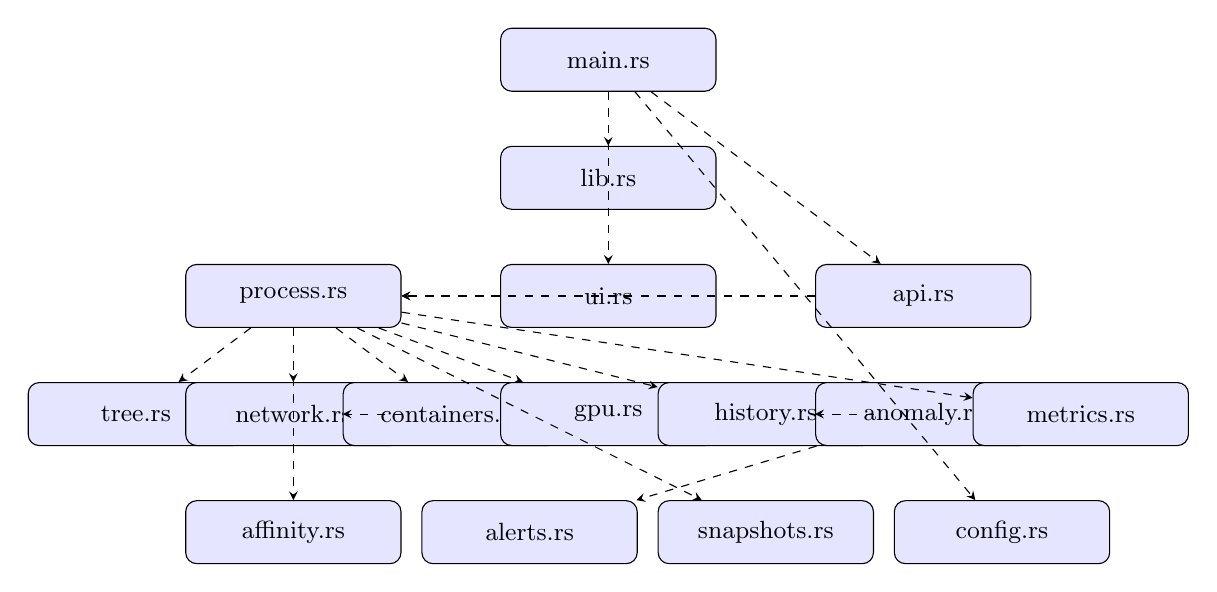
\begin{tikzpicture}[
    module/.style={rectangle, draw, fill=blue!10, text width=2.5cm, text centered, rounded corners, minimum height=0.8cm, font=\small},
    depends/.style={->, >=stealth, dashed}
]

% Core modules
\node[module] (main) at (6,0) {main.rs};
\node[module] (lib) at (6,-1.5) {lib.rs};

% Primary modules
\node[module] (process) at (2,-3) {process.rs};
\node[module] (ui) at (6,-3) {ui.rs};
\node[module] (api) at (10,-3) {api.rs};

% Secondary modules (left)
\node[module] (tree) at (0,-4.5) {tree.rs};
\node[module] (network) at (2,-4.5) {network.rs};
\node[module] (containers) at (4,-4.5) {containers.rs};

% Secondary modules (middle)
\node[module] (gpu) at (6,-4.5) {gpu.rs};
\node[module] (history) at (8,-4.5) {history.rs};

% Secondary modules (right)
\node[module] (anomaly) at (10,-4.5) {anomaly.rs};
\node[module] (metrics) at (12,-4.5) {metrics.rs};

% Utility modules
\node[module] (affinity) at (2,-6) {affinity.rs};
\node[module] (alerts) at (5,-6) {alerts.rs};
\node[module] (snapshots) at (8,-6) {snapshots.rs};
\node[module] (config) at (11,-6) {config.rs};

% Dependencies
\draw[depends] (main) -- (lib);
\draw[depends] (main) -- (ui);
\draw[depends] (main) -- (api);

\draw[depends] (ui) -- (process);
\draw[depends] (api) -- (process);

\draw[depends] (process) -- (tree);
\draw[depends] (process) -- (network);
\draw[depends] (process) -- (containers);
\draw[depends] (process) -- (gpu);
\draw[depends] (process) -- (history);

\draw[depends] (network) -- (containers);
\draw[depends] (history) -- (anomaly);
\draw[depends] (process) -- (metrics);

\draw[depends] (anomaly) -- (alerts);
\draw[depends] (process) -- (affinity);
\draw[depends] (process) -- (snapshots);
\draw[depends] (main) -- (config);

\end{tikzpicture}
\caption{Module Dependency Graph}
\label{fig:modules}
\end{figure}

\subsection{Module Descriptions}

\begin{table}[H]
\centering
\caption{Module Descriptions and Responsibilities}
\label{tab:modules}
\small
\begin{tabularx}{\textwidth}{|l|l|X|}
\hline
\textbf{Module} & \textbf{Lines} & \textbf{Responsibilities} \\
\hline
main.rs & 317 & Entry point, CLI parsing, mode selection \\
\hline
lib.rs & 132 & Public API exports, library interface \\
\hline
process.rs & 508 & Process enumeration, monitoring, control \\
\hline
ui.rs & 664 & Terminal UI, event handling, rendering \\
\hline
tree.rs & 187 & Process tree building, hierarchy \\
\hline
network.rs & 346 & Network connections, container basics \\
\hline
gpu.rs & 286 & Multi-vendor GPU monitoring \\
\hline
history.rs & 341 & SQLite storage, time-series queries \\
\hline
api.rs & 436 & REST API endpoints, HTTP server \\
\hline
metrics.rs & 342 & Prometheus/InfluxDB export \\
\hline
anomaly.rs & 460 & Statistical analysis, anomaly detection \\
\hline
logging.rs & 252 & Structured logging, tracing \\
\hline
affinity.rs & 333 & CPU affinity, nice values \\
\hline
alerts.rs & 445 & Alert rules, notifications \\
\hline
snapshots.rs & 296 & State capture, comparison \\
\hline
groups.rs & 164 & Process groups, sessions \\
\hline
memmap.rs & 342 & Memory map parsing, visualization \\
\hline
profiles.rs & 440 & Saved view configurations \\
\hline
diffing.rs & 235 & Process state diffing \\
\hline
containers.rs & 403 & Enhanced container detection \\
\hline
config.rs & 327 & Configuration management \\
\hline
\textbf{Total} & \textbf{7,730} & \\
\hline
\end{tabularx}
\end{table}

\section{Key Data Structures}

\subsection{ProcessInfo Structure}

Core data structure representing a process:

\begin{lstlisting}[caption={ProcessInfo Structure},label={lst:processinfo}]
pub struct ProcessInfo {
    pub pid: u32,              // Process ID
    pub ppid: u32,             // Parent process ID
    pub name: String,          // Process name (from comm)
    pub command: String,       // Full command line
    pub user: String,          // Owner username
    pub uid: u32,              // User ID
    pub gid: u32,              // Group ID

    // Resource metrics
    pub cpu_usage: f32,        // CPU percentage
    pub memory_usage: u64,     // Memory in bytes
    pub memory_percent: f32,   // Memory percentage

    // State information
    pub status: String,        // R/S/D/Z/T
    pub priority: i32,         // Priority value
    pub nice: i32,             // Nice value
    pub threads: u32,          // Thread count

    // Timing
    pub start_time: u64,       // Start time (timestamp)
    pub running_time: Duration, // Elapsed time

    // Extended features
    pub network_connections: Option<usize>,
    pub is_container: bool,
    pub container_id: Option<String>,
    pub cgroup_memory_limit: Option<u64>,
    pub gpu_memory: Option<u64>,
}
\end{lstlisting}

\subsection{Process Tree Node}

Hierarchical structure for tree view:

\begin{lstlisting}[caption={ProcessNode Structure}]
pub struct ProcessNode {
    pub process: ProcessInfo,      // Process data
    pub children: Vec<ProcessNode>, // Child processes
    pub level: usize,              // Tree depth
}
\end{lstlisting}

\subsection{Historical Data Records}

Time-series storage schema:

\begin{lstlisting}[caption={Historical Data Schema},language=SQL]
CREATE TABLE process_history (
    id INTEGER PRIMARY KEY,
    timestamp INTEGER NOT NULL,
    pid INTEGER NOT NULL,
    name TEXT NOT NULL,
    cpu_percent REAL NOT NULL,
    memory_kb INTEGER NOT NULL,
    user TEXT NOT NULL,
    INDEX idx_timestamp (timestamp),
    INDEX idx_pid (pid)
);

CREATE TABLE system_history (
    id INTEGER PRIMARY KEY,
    timestamp INTEGER NOT NULL,
    total_cpu_percent REAL NOT NULL,
    total_memory_kb INTEGER NOT NULL,
    process_count INTEGER NOT NULL,
    INDEX idx_timestamp (timestamp)
);
\end{lstlisting}

\subsection{Alert Rule Structure}

Configuration for alert conditions:

\begin{lstlisting}[caption={AlertRule Structure}]
pub struct AlertRule {
    pub enabled: bool,
    pub alert_type: AlertType,  // HighCpu, HighMemory, etc.
    pub threshold: f64,         // Trigger threshold
    pub duration_secs: u64,     // Sustained duration
    pub cooldown_secs: u64,     // Time between alerts
    pub process_filter: Option<String>, // Process pattern
}

pub enum AlertType {
    HighCpu,
    HighMemory,
    ProcessCount,
    Custom(String),
}
\end{lstlisting}

\section{Concurrency Model}

\subsection{Async Architecture}

The system employs Tokio async runtime for I/O-bound operations while using synchronous code for CPU-bound tasks.

\begin{figure}[H]
\centering
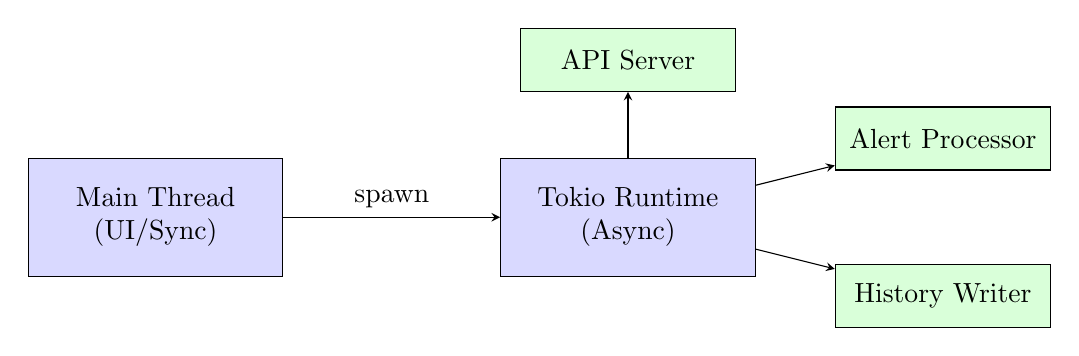
\begin{tikzpicture}[
    thread/.style={rectangle, draw, fill=blue!15, text width=3cm, text centered, minimum height=1.5cm},
    task/.style={rectangle, draw, fill=green!15, text width=2.5cm, text centered, minimum height=0.8cm},
    arrow/.style={->, >=stealth}
]

% Main thread
\node[thread] (main) at (0,0) {Main Thread\\(UI/Sync)};

% Tokio runtime
\node[thread] (tokio) at (6,0) {Tokio Runtime\\(Async)};

% Tasks
\node[task] (api) at (6,2) {API Server};
\node[task] (alerts) at (10,1) {Alert Processor};
\node[task] (history) at (10,-1) {History Writer};

% Arrows
\draw[arrow] (main) -- node[above] {spawn} (tokio);
\draw[arrow] (tokio) -- (api);
\draw[arrow] (tokio) -- (alerts);
\draw[arrow] (tokio) -- (history);

\end{tikzpicture}
\caption{Concurrency Model}
\label{fig:concurrency}
\end{figure}

\subsection{Thread Safety}

\begin{itemize}[leftmargin=*]
    \item \textbf{UI Thread}: Single-threaded event loop (ratatui)
    \item \textbf{API Server}: Multi-threaded request handling (Actix-web workers)
    \item \textbf{Alert Processor}: Background async task
    \item \textbf{History Writer}: Periodic async task
    \item \textbf{Synchronization}: Arc<Mutex<T>> for shared state
\end{itemize}

\subsection{Data Flow Diagram}

\begin{figure}[H]
\centering
\begin{tikzpicture}[
    process/.style={ellipse, draw, fill=blue!10, text width=2cm, text centered, minimum height=1cm},
    data/.style={rectangle, draw, fill=yellow!10, text width=2cm, text centered},
    arrow/.style={->, >=stealth, thick}
]

\node[data] (proc) at (0,0) {/proc/*};
\node[process] (scan) at (3,0) {Scan Processes};
\node[data] (list) at (6,0) {Process List};

\node[process] (enrich) at (6,-2) {Enrich Data\\(GPU, Network)};
\node[data] (enriched) at (6,-4) {Enriched List};

\node[process] (analyze) at (3,-4) {Analyze};
\node[process] (display) at (9,-4) {Display};

\node[data] (history) at (3,-6) {History DB};
\node[data] (alerts) at (6,-6) {Alert Queue};
\node[data] (ui) at (9,-6) {Terminal};

\draw[arrow] (proc) -- (scan);
\draw[arrow] (scan) -- (list);
\draw[arrow] (list) -- (enrich);
\draw[arrow] (enrich) -- (enriched);
\draw[arrow] (enriched) -- (analyze);
\draw[arrow] (enriched) -- (display);
\draw[arrow] (analyze) -- (history);
\draw[arrow] (analyze) -- (alerts);
\draw[arrow] (display) -- (ui);

\end{tikzpicture}
\caption{Data Flow from /proc to Display}
\label{fig:dataflow}
\end{figure}

\section{Design Patterns}

\subsection{Builder Pattern}

Configuration objects use builder pattern:

\begin{lstlisting}[caption={Builder Pattern Example}]
let config = LogConfig::builder()
    .level(Level::INFO)
    .log_to_file(true)
    .log_file_path("/var/log/pm.log")
    .json_format(false)
    .rotation(LogRotation::Daily)
    .build()?;
\end{lstlisting}

\subsection{Strategy Pattern}

Pluggable exporters for metrics:

\begin{lstlisting}[caption={Strategy Pattern - Metrics Export}]
pub trait MetricsExporter {
    fn export(&self, processes: &[ProcessInfo]) -> String;
}

pub struct PrometheusExporter;
pub struct InfluxDBExporter;

impl MetricsExporter for PrometheusExporter {
    fn export(&self, processes: &[ProcessInfo]) -> String {
        // Prometheus format
    }
}
\end{lstlisting}

\subsection{Observer Pattern}

Alert system observes process state changes:

\begin{lstlisting}[caption={Observer Pattern - Alerts}]
pub struct AlertManager {
    rules: Vec<AlertRule>,
    tx: mpsc::Sender<Alert>,
}

impl AlertManager {
    pub async fn check_process(&mut self,
                                pid: u32,
                                name: &str,
                                cpu: f32,
                                mem: f32) {
        for rule in &self.rules {
            if rule.matches(cpu, mem) {
                self.tx.send(Alert::new(rule, pid)).await;
            }
        }
    }
}
\end{lstlisting}

\subsection{Repository Pattern}

Data access abstraction:

\begin{lstlisting}[caption={Repository Pattern - History}]
pub struct HistoryRepository {
    db: Connection,
}

impl HistoryRepository {
    pub fn save_process(&self, entry: ProcessHistoryEntry)
        -> Result<()> { ... }

    pub fn query_range(&self, start: i64, end: i64)
        -> Result<Vec<ProcessHistoryEntry>> { ... }
}
\end{lstlisting}

\section{Error Handling Strategy}

\subsection{Error Types}

Custom error hierarchy using thiserror:

\begin{lstlisting}[caption={Error Type Hierarchy}]
use thiserror::Error;

#[derive(Error, Debug)]
pub enum ProcessManagerError {
    #[error("Process not found: {0}")]
    ProcessNotFound(u32),

    #[error("Permission denied for process {0}")]
    PermissionDenied(u32),

    #[error("Failed to read /proc: {0}")]
    ProcReadError(String),

    #[error("Database error: {0}")]
    DatabaseError(#[from] rusqlite::Error),

    #[error("IO error: {0}")]
    IoError(#[from] std::io::Error),
}
\end{lstlisting}

\subsection{Error Propagation}

Using Result<T, E> for explicit error handling:

\begin{lstlisting}[caption={Error Propagation}]
pub fn get_process_info(pid: u32) -> Result<ProcessInfo> {
    let stat = read_proc_stat(pid)?;  // Propagate error
    let status = read_proc_status(pid)?;

    Ok(ProcessInfo {
        pid,
        name: parse_name(&stat)?,
        // ...
    })
}
\end{lstlisting}

\subsection{Graceful Degradation}

Optional features use Option<T>:

\begin{lstlisting}[caption={Graceful Degradation}]
// GPU monitoring is optional
pub fn enrich_with_gpu(info: &mut ProcessInfo) {
    info.gpu_memory = get_gpu_memory(info.pid).ok();
    // If GPU detection fails, field is None
}
\end{lstlisting}

\section{Performance Optimizations}

\subsection{Caching Strategy}

\begin{itemize}[leftmargin=*]
    \item \textbf{User Cache}: Map UID to username once per refresh
    \item \textbf{GPU Cache}: Cache nvidia-smi output for 1 second
    \item \textbf{Network Cache}: Cache /proc/net/tcp parsing
\end{itemize}

\subsection{Lazy Evaluation}

\begin{lstlisting}[caption={Lazy Evaluation}]
pub struct ProcessInfo {
    // ... other fields ...

    // Expensive to compute, only when needed
    network_connections: Option<usize>,
    gpu_memory: Option<u64>,
}

// Computed on-demand
pub fn get_network_connections(&mut self) -> usize {
    if self.network_connections.is_none() {
        self.network_connections =
            Some(count_connections(self.pid));
    }
    self.network_connections.unwrap()
}
\end{lstlisting}

\subsection{Batch Processing}

Process /proc entries in batches to improve cache locality.

\section{Security Architecture}

\subsection{Privilege Separation}

\begin{figure}[H]
\centering
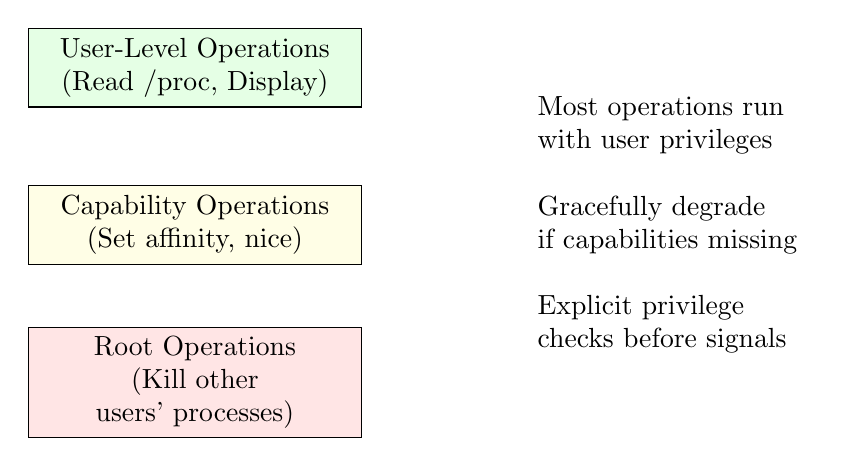
\begin{tikzpicture}[
    level/.style={rectangle, draw, fill=blue!10, text width=4cm, text centered, minimum height=1cm},
    arrow/.style={->, >=stealth}
]

\node[level, fill=green!10] (user) at (0,0) {User-Level Operations\\(Read /proc, Display)};
\node[level, fill=yellow!10] (cap) at (0,-2) {Capability Operations\\(Set affinity, nice)};
\node[level, fill=red!10] (root) at (0,-4) {Root Operations\\(Kill other users' processes)};

\node[draw=none] (note) at (6,-2) {
    \begin{tabular}{l}
    Most operations run \\
    with user privileges \\
    \\
    Gracefully degrade \\
    if capabilities missing \\
    \\
    Explicit privilege \\
    checks before signals
    \end{tabular}
};

\end{tikzpicture}
\caption{Privilege Separation Model}
\label{fig:privileges}
\end{figure}

\subsection{Input Validation}

All user inputs validated:

\begin{lstlisting}[caption={Input Validation}]
pub fn set_nice_value(pid: u32, nice: i32) -> Result<()> {
    // Validate range
    if nice < -20 || nice > 19 {
        return Err(Error::InvalidNiceValue(nice));
    }

    // Verify process exists and owned by user
    verify_process_ownership(pid)?;

    // Safe to proceed
    unsafe {
        libc::setpriority(libc::PRIO_PROCESS, pid, nice);
    }
    Ok(())
}
\end{lstlisting}

\section{Summary}

This chapter presented the architectural design of the Linux Process Manager, including:

\begin{itemize}[leftmargin=*]
    \item Modular, layered architecture with clear separation of concerns
    \item 20 specialized modules totaling 7,730 lines of code
    \item Async concurrency model using Tokio runtime
    \item Comprehensive data structures for process representation
    \item Design patterns (Builder, Strategy, Observer, Repository)
    \item Robust error handling with custom error types
    \item Performance optimizations (caching, lazy evaluation)
    \item Security-conscious design with privilege separation
\end{itemize}

The next chapter details the implementation of these architectural components.
